\chapter{Analisis}
\label{chap:analisis}

Bab ini membahas tentang cara kerja algoritma \textit{backtracking} dan algoritma \textit{hybrid genetic} untuk menyelesaikan permainan teka-teki Calcudoku.

\section{Algoritma \textit{Backtracking}}
\label{sec:analisisbt}

Untuk mengilustrasikan cara kerja algoritma \textit{backtracking}, akan digunakan permainan teka-teki Calcudoku yang digambarkan pada Gambar~\ref{fig:analisisbt1} sebagai contoh.

\begin{figure}
\centering
\captionsetup{justification=centering}
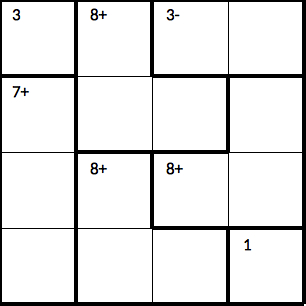
\includegraphics[scale=0.5]{Gambar/backtracking/State1}
\caption[Contoh permainan teka-teki Calcudoku dengan ukuran \textit{grid} 4 x 4 yang belum diselesaikan, seperti yang digambarkan pada Gambar~\ref{fig:backtracking1}.  ~\cite{fahda:16:backtracking}]{Contoh permainan teka-teki dengan ukuran \textit{grid} 4 x 4 yang belum diselesaikan, seperti yang digambarkan pada Gambar ~\ref{fig:backtracking1}.  ~\cite{fahda:16:backtracking}}
\label{fig:analisisbt1}
\end{figure}

\begin{enumerate}
\item Algoritma \textit{backtracking} dimulai dengan teka-teki yang belum diselesaikan, seperti yang digambarkan pada Gambar~\ref{fig:analisisbt1} (\textit{state} 1).
\item Algoritma mengisikan sel pada baris ke-1 dan kolom ke-1 dengan angka 1 (\textit{state} 2), tetapi angka 1 tidak sesuai dengan angka tujuan dari \textit{cage} tersebut.
\item Algoritma lalu mencoba kemungkinan angka berikutnya, yaitu angka 2 (\textit{state} 3), tetapi angka 2 juga tidak sesuai dengan angka tujuan dari \textit{cage} tersebut.
\item Algoritma lalu mencoba kemungkinan angka berikutnya, yaitu angka 3 (\textit{state} 4), seperti dapat dilihat di Gambar ~\ref{fig:analisisbt2}, dan ternyata angka 3 sesuai dengan angka tujuan dari \textit{cage} tersebut, sehingga algoritma dapat maju ke sel berikutnya.

\begin{figure}
\centering
\captionsetup{justification=centering}
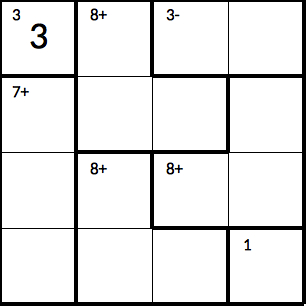
\includegraphics[scale=0.5]{Gambar/backtracking/State4}
\caption[\textit{State} 4]{\textit{State} 4}
\label{fig:analisisbt2}
\end{figure}

\item Algoritma lalu mengisikan sel pada baris ke-1 dan kolom ke-2 dengan angka 1 (\textit{state} 5). Algoritma lalu maju ke sel berikutnya.
\item Algoritma lalu mengisikan sel pada baris ke-1 dan kolom ke-3 dengan angka 1 (\textit{state} 6), tetapi angka 1 sudah pernah digunakan dalam baris tersebut.
\item Algoritma lalu mencoba kemungkinan angka berikutnya, yaitu angka 2 (\textit{state} 7). Algoritma lalu maju ke sel berikutnya.
\item Algoritma lalu mengisikan sel pada baris ke-1 dan kolom ke-4 dengan angka 1 (\textit{state} 8), tetapi angka 1 sudah pernah digunakan dalam baris tersebut.
\item Algoritma lalu mencoba kemungkinan angka berikutnya, yaitu angka 2 (\textit{state} 9), tetapi angka 2 sudah pernah digunakan dalam baris tersebut.
\item Algoritma lalu mencoba kemungkinan angka berikutnya, yaitu angka 3 (\textit{state} 10), tetapi angka 3 sudah pernah digunakan dalam baris tersebut.
\item Algoritma lalu mencoba kemungkinan angka berikutnya, yaitu angka 4 (\textit{state} 11), seperti dapat dilihat di Gambar ~\ref{fig:analisisbt3}, tetapi hasilnya tidak sesuai dengan angka tujuan dari \textit{cage} tersebut.

\begin{figure}
\centering
\captionsetup{justification=centering}
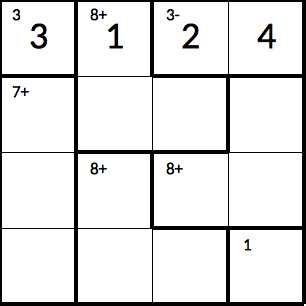
\includegraphics[scale=0.5]{Gambar/backtracking/State11}
\caption[\textit{State} 11]{\textit{State} 11}
\label{fig:analisisbt3}
\end{figure}

\item Karena semua kemungkinan angka untuk baris ke-1 dan kolom ke-4 telah dicoba dan gagal, maka algoritma harus mundur kembali ke (\textit{state} 7). Algoritma mencoba kemungkinan angka berikutnya, yaitu angka 3  (\textit{state} 12), seperti dapat dilihat di Gambar ~\ref{fig:analisisbt4}, tetapi angka 3 sudah pernah digunakan dalam baris tersebut. Algoritma lalu maju ke sel berikutnya.

\begin{figure}
\centering
\captionsetup{justification=centering}
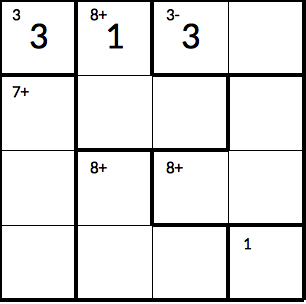
\includegraphics[scale=0.5]{Gambar/backtracking/State12}
\caption[\textit{State} 12]{\textit{State} 12}
\label{fig:analisisbt4}
\end{figure}

\item Algoritma lalu mencoba kemungkinan angka berikutnya, yaitu angka 4 (\textit{state} 13). Algoritma lalu maju ke sel berikutnya.
\item Algoritma lalu mengisikan sel pada baris ke-1 dan kolom ke-4 dengan angka 1 (\textit{state} 14), tetapi angka 1 sudah pernah digunakan dalam baris tersebut.
\item Algoritma lalu mencoba kemungkinan angka berikutnya, yaitu angka 2 (\textit{state} 15), tetapi hasilnya tidak sesuai dengan angka tujuan dari \textit{cage} tersebut.
\item Algoritma lalu mencoba kemungkinan angka berikutnya, yaitu angka 3 (\textit{state} 16), tetapi angka 3 sudah pernah digunakan dalam baris tersebut.
\item Algoritma lalu mencoba kemungkinan angka berikutnya, yaitu angka 4 (\textit{state} 17), seperti dapat dilihat di Gambar ~\ref{fig:analisisbt5}, tetapi angka 4 sudah pernah digunakan dalam baris tersebut.

\begin{figure}
\centering
\captionsetup{justification=centering}
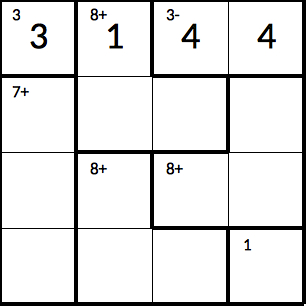
\includegraphics[scale=0.5]{Gambar/backtracking/State17}
\caption[\textit{State} 17]{\textit{State} 17}
\label{fig:analisisbt5}
\end{figure}

\item Karena semua kemungkinan angka untuk baris ke-1 dan kolom ke-3 dan ke-4 telah dicoba dan gagal, maka algoritma harus mundur kembali ke (\textit{state} 5). Algoritma mencoba kemungkinan angka berikutnya, yaitu angka 2  (\textit{state} 18), seperti dapat dilihat di Gambar ~\ref{fig:analisisbt6}. Algoritma lalu maju ke sel berikutnya.

\begin{figure}
\centering
\captionsetup{justification=centering}
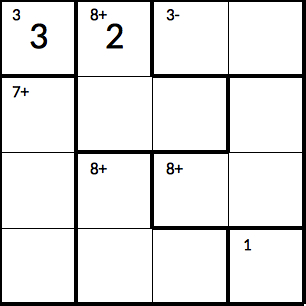
\includegraphics[scale=0.5]{Gambar/backtracking/State18}
\caption[\textit{State} 18]{\textit{State} 18}
\label{fig:analisisbt6}
\end{figure}

\item Algoritma lalu mengisikan sel pada baris ke-1 dan kolom ke-3 dengan angka 1 (\textit{state} 19), seperti dapat dilihat di Gambar ~\ref{fig:analisisbt7}. Algoritma lalu maju ke sel berikutnya.

\begin{figure}
\centering
\captionsetup{justification=centering}
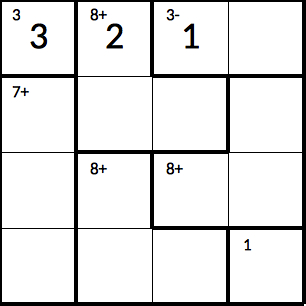
\includegraphics[scale=0.5]{Gambar/backtracking/State19}
\caption[\textit{State} 19]{\textit{State} 19}
\label{fig:analisisbt7}
\end{figure}

\item Algoritma lalu mengisikan sel pada baris ke-1 dan kolom ke-4 dengan angka 1 (\textit{state} 20), tetapi angka 1 sudah pernah digunakan dalam baris tersebut.
\item Algoritma lalu mencoba kemungkinan angka berikutnya, yaitu angka 2 (\textit{state} 21), tetapi angka 2 sudah pernah digunakan dalam baris tersebut.
\item Algoritma lalu mencoba kemungkinan angka berikutnya, yaitu angka 3 (\textit{state} 22), tetapi angka 3 sudah pernah digunakan dalam baris tersebut.
\item Algoritma lalu mencoba kemungkinan angka berikutnya, yaitu angka 4 (\textit{state} 23), dan ternyata hasilnya sesuai dengan angka tujuan dari \textit{cage} tersebut, seperti dapat dilihat di Gambar ~\ref{fig:analisisbt8}. Algoritma telah selesai mengisikan baris ke-1, sehingga bisa maju ke baris berikutnya.

\begin{figure}
\centering
\captionsetup{justification=centering}
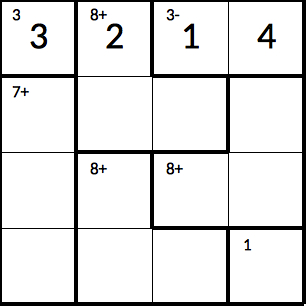
\includegraphics[scale=0.5]{Gambar/backtracking/State23}
\caption[\textit{State} 23]{\textit{State} 23}
\label{fig:analisisbt8}
\end{figure}

\end{enumerate}